\chapter{System Architecture and Design}\label{chap:system_architecture_rewrite}

The previous Chapter~\ref{chap:background} defined the technical background for scene-aware dialogue on Pepper; 
This chapter describes how these ideas are organized in the implemented system in a high-level view before the individual parts are described in detail. The server-side architecture is described in Chapter~\ref{chap:server_side_rewrite}, and the robot client is described in Chapter~\ref{chap:robot_side_rewrite}. The code is publicly available at \url{https://github.com/JakubCiesko/pepper-ot}.

The system follows a distributed client-server design. Pepper is used as an interaction platform, while a separate server performs the computationally expensive perception, scene memory managment, and language processing. This choice follows directly from the motivation in Chapter~\ref{chap:intro}, where related Pepper systems were shown to rely on cloud or remote processing for modern perception and language components~\cite{reyes_near_2018,wilson_enhancing_2025,becerra_improving_2024,brad_retrieval-augmented_2025,hafez_enhancing_nodate,grassi_grounding_2024,latif_physicsassistant_2024,trinquet_future_2025}. 
It is also supported by the Pepper platform presentation in Section~\ref{sec:pepper-platform}; Pepper provides useful interaction hardware and NAOqi services, but its resources are limited for a full or even a partial vision and language pipeline.

\begin{figure}[t]
\centering
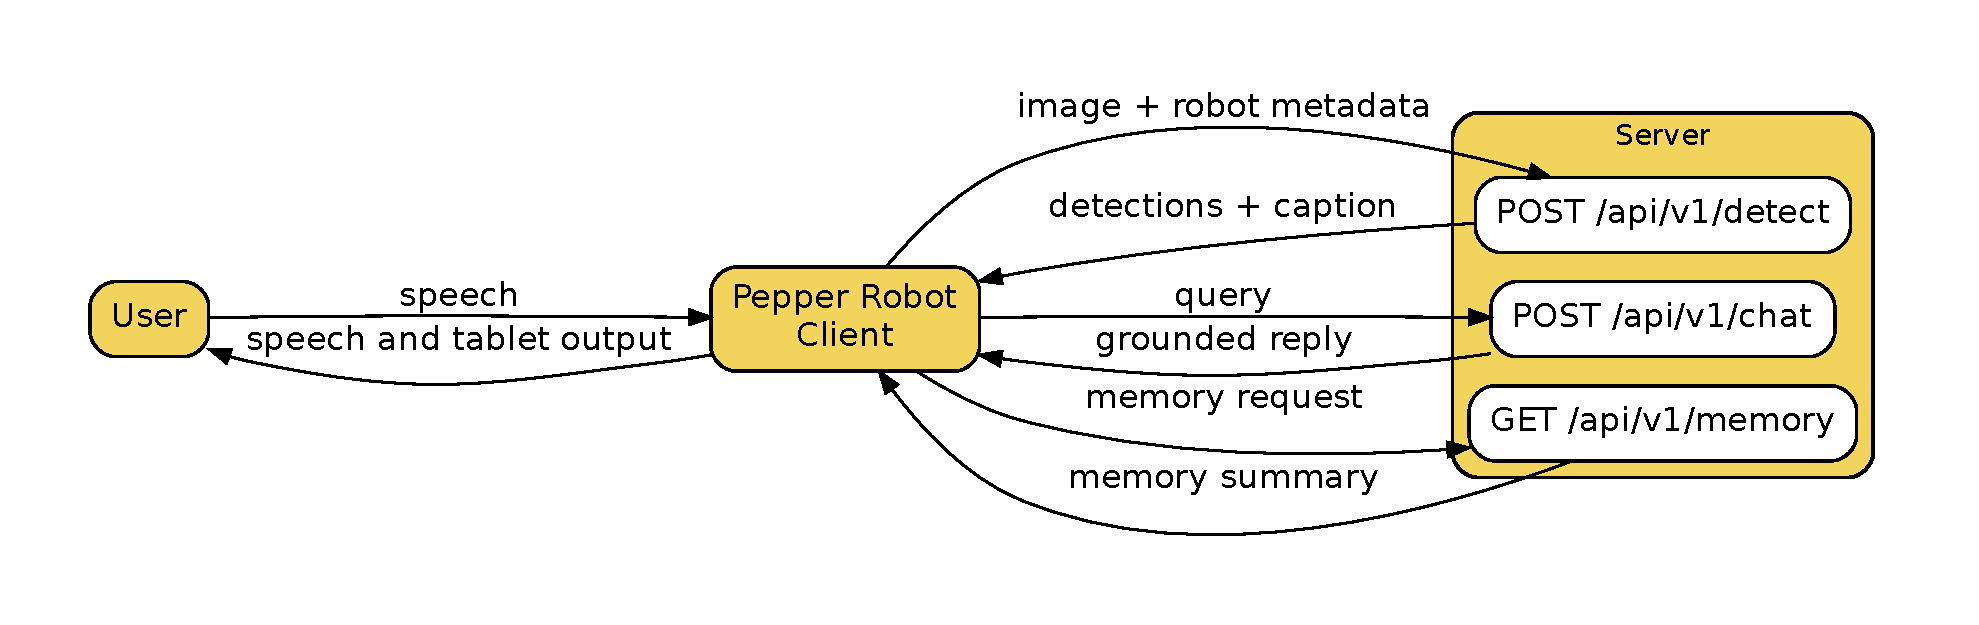
\includegraphics[width=1\linewidth]{pics/architecture.pdf}
\caption{High-level architecture of the proposed scene-aware dialogue system. The Pepper robot (client) handles user speech input, speech and tablet output, image capture, and robot metadata collection. The server exposes perception, chat, and memory endpoints that create and use the scene representation.}
\label{fig:overall-system-architecture}
\end{figure}

Figure~\ref{fig:overall-system-architecture} shows the main information flow. The user interacts with Pepper through speech. The robot client sends an image and robot metadata to the server when prompted for a scan of its surroundings based on QiChat grammar. When the user asks a question, it sends the text queries to the server's chat endpoint. It can also request a memory summary when the user wants to inspect what the system currently remembers. The server answers all these requests through a small set of HTTP endpoints and returns detections, captions, grounded replies, or memory summaries. These are then furhter processed or presented to the user using its native TTS module.

The robot side is generally responsible for the parts of the system that provide data for processing or must stay close to the user. 
It runs inside Pepper's NAOqi application environment as a NAOqi service which listens through QiChat, moves the head during scans, captures images, speaks answers, and updates the tablet. It also keeps remembered object labels, their relationship and attributes, and cached pregenerated question-answer pairs for fast answerings without calling the server. 

The server side owns the heavier and more persistent part of the system. 
It receives robot observations, runs object detection, associates detections with remembered objects, generates captions, builds scene graph relations, updates scene memory, and calls language models for grounded responses. 
The server also exposes a dashboard which servers as a configuration interface for development and changing the pipeline settings as well as monitoring device displaying the processed scene representation. %This makes the server the central place where visual observations become a structured representation that can be used in dialogue.

The shared boundary between the two sides is intentionally simple. Visual requests contain image bytes and a metadata payload with head pose, camera field of view, image size, frame identifiers, scan identifiers, visible people and available social signals captured by NAOqi APIs, i. e. ALPeoplePerception. 
Dialogue requests contain a query, an optional conversation identifier, language information, and sometimes an object label. These contracts keep the robot client independent of the exact detector, caption model, scene graph method, or language model used by the server and make it easy for swap of these components.

The architecture uses different interaction modes both for detection and for conversation. The robot is able to take just a quick look or do a full scan of its surroundings. A quick look can request a caption and optionally refresh visual memory in the background. A scan moves Pepper's head through several poses and sends multiple observations for detection. A general question can use the existing scene memory without taking a new picture. An object-focused question sends an object label so that the server can build a narrower context from matching objects and their relations. A memory request returns a compact summary displayed on the tablet and populates QiChat dynamic concepts.

Scene memory serves as the main abstraction between perception and conversation. Raw detections are tied to one image, while dialogue usually needs stable references over time. The server therefore stores tracked objects, their identifiers, attributes, relations, recent captions, timestamps, and object crops. The robot client only mirrors the parts needed for interaction, such as labels and cached questions. MAYBEDROP: This separation avoids two competing world models and gives the dialogue layer one authoritative source of scene state.

MAYBEDROP KEEP JUST LAST SENTENCE: The server-client split also supports reliability. The robot client can reject overlapping turns, speak localized fallback messages, and recover from camera or network errors. The server can isolate heavy inference in a worker process and expose its internal state through the dashboard. The result is a system where Pepper remains responsive as an interaction device, while the external server provides the computational capacity needed for scene-aware dialogue.
